\documentclass[11pt,a4paper,twocolumn]{scrartcl}
\usepackage{mathptmx}
\usepackage{amsmath}
\usepackage{amsthm}
\usepackage[T1]{fontenc}
\usepackage[bitstream-charter]{mathdesign}
\usepackage{sectsty}
\usepackage[activate={true,nocompatibility},final,kerning=true,spacing=true,factor=1100,stretch=10,shrink=10]{microtype}
\usepackage[backend=biber,style=numeric,sorting=none,isbn=false,backref=false]{biblatex}
\usepackage{mdframed}
\usepackage[font=small,labelfont=bf,margin=25pt]{caption}
\usepackage{easy-todo}
\usepackage[usenames,dvipsnames,table]{xcolor}
\usepackage{colortbl}
\usepackage{listings}
\usepackage{graphicx}
\usepackage{multirow}
\usepackage[hang,flushmargin]{footmisc}
\usepackage{enumitem}
\usepackage{fancyvrb}
\usepackage{changepage}
\usepackage{setspace}
\usepackage{array}
\usepackage[hidelinks]{hyperref}
\usepackage{booktabs}
\usepackage{tabularx}
\usepackage{rotating}
\usepackage{url}
\usepackage[section]{placeins}
\usepackage{newfloat}
\usepackage{comment}
\usepackage{url}

%\usepackage[top=1in, bottom=1in, left=1.5in, right=1.5in]{geometry} % Margins

\urlstyle{same}

\setkomafont{disposition}{\normalfont\bfseries}

\addbibresource{MG.bib}

\microtypecontext{spacing=nonfrench}

\newcolumntype{C}[1]{>{\centering\arraybackslash}p{#1}}

\renewcommand{\labelitemi}{$\triangleright$}
\renewcommand{\labelitemii}{$\bullet$}

%------------------------------------------------------------------------

\title{The Computer Cannot Flip the Board: A Genetic Algorithm for Playing Monopoly}
\author{Benjamin Pring}

\begin{document}

\maketitle

\begin{abstract}
\noindent \textbf{Abstract} We evaluate of the capability for a genetic algorithm to learn to play games, in this case the Parker Brothers' \textit{Monopoly} board game. Monopoly was selected as it is largely based on the luck of the dice, however there are a few important decisions the player is required to make, in particular which properties to buy, sell or trade when the opportunity arises. These are the decisions to which we can test the fitness of the genetic approach. We describe our approach to implementing a simple simulator; then test the effects of varying the parameters of the algorithm.

\vspace{2em}

\noindent \textbf{Keywords} Genetic Algorithms, AI, Game Theory, Monopoly
\end{abstract}

%----------------------------------------------------------------------------------------------------

\section{Introduction}

\subsubsection*{Author's note}

As the title suggests, please note that this research is to be taken with more than a grain of salt. The project started as a small programming exercise, however seemed worth translating into an article such that others might enjoy some of the concepts involved -- we hope you find yourself in this category!

\subsection{Genetic Algorithms}

Genetic algorithms (GAs) are a class of artificial intelligence heuristic, in which the approach is to emulate natural selection in order to generate optimized solutions to a given problem~\cite{mitchell1998introduction}. Genetic algorithms have a relatively long history, going back to the mid nineteenth century to work by Alex Fraser~\cite{fraser1960simulation} and Bremermann~\cite{bremermann1962optimization}. 

The typical approach of a genetic algorithm is to use the processes of evolution by natural selection -- that is \textit{selection} itself, \textit{inheritance}, \textit{mutation}, and \textit{crossover} -- in order to train `individuals' over a series of generations so that they solve problems more effectively. In order to do this, the parameters by which behaviour or form (phenotype) differ between individuals are defined by some form of code (genotype). The algorithm thus runs along the following lines: 

\begin{enumerate}
\item From a general population, multiple phenotypes that performed well within the problem space are selected, those that did not perform well are removed.
\item Within the group of succesful individuals, genotypes are mixed according to some crossover strategy. 
\item Some degree of mutation is also applied to the genotypes.
\item The genotypes produced by these steps are inherited by new individuals which are returned to the population.
\end{enumerate}

In many classes of problems, one of the main limitations of genetic algorithms is that they must perform some function to evaluate the success of every individual to provide a basis for selection. It is important for a genetic algorithm to run over many generations and on a reasonably large population in order to succesfully train; this can result is the fitness function being run a large number of times. Fortunately in most game-playing problems, we can establish the fitness of an individual simply by their winning the game. We just need to run simulations of the game over and over, pitting several individuals against each other each time, and then selecting the winner.

\subsection{Monopoly}

Originally popularised by the Parker Brothers in the early twentieth century, \textit{Monopoly} is a board game in which players must accrue wealth and property in order to drive the other players out of business. It is by no means a complicated game, indeed much is decided by chance, and once a player establishes a lead, it is unlikely they will fail to win. This is likely the reason that, in our experience, most games of monopoly end with a bad humour between the players, the winner is often abandoned to pack up the pieces, which on some occasions will have been scattered from the table. Typically the game comes to an abrupt end when a player lands on a rival's newly built, high-rent hotel, or when the red backs of mortgaged properties begin to signal the endgame. In fact by some analyses, the modern game less about fun, but instead about the pitfalls of unregulated capitalism~\cite{ender2004modified}. However, for the purposes of learning about genetic algorithms and testing some theories in this area, we believe it is relatively well suited for the following reasons: 

\begin{itemize}

\item The game is short, decisive and largely deterministic, which make it easy to simulate on a computer 
\item No great amount of strategy or teamwork are required, which we would like to put outside the scope of this investigation of artificial intelligence 
\item Relatively few but significant decisions need to made. 
\item The game is widely understood, but as experienced players will testify, there are a few key strategies that can help secure victory. This will allow us to provide some qualitative evaluation of the result of our experiments.
\item Last but not least, the computer, devoid of emotion, is up for playing countless games until the bitter end, without flipping the board or storming off in frustration.

\end{itemize}

For the purposes of this project, we shall be using the UK English layout of the Monopoly board, rather than the original US edition. This was done simply for familiarity's sake, the results are directly translatable into any of the (many, many) other editions of the board.

\subsection{This article}

In this article, we first describe the implementation of our simulation, including how we have programmed the rules of the game and the methods used to develop the genetic algorithm. We then go on to show some results of our GA, along with some discussion and a look at how outcomes vary with changes to the conditions and switches of the simulation. Finally, we draw some conclusions and suggest at future extensions.

%----------------------------------------------------------------------------------------------------
\section{Implementation}
\label{sec:imp}

In this section we cover a few key areas of the implementation and method of our experiments.

\subsection{Rules of the Game}

The version of the rules of Monopoly that we have used to implement the game are something close to the standard rules as defined by the instruction manual provided with the 2007 edition of the game, and are this not listed in full here. We assume that most readers will have a reasonable knowledge of many of the game concepts, however reading these instructions is actually recommended to any occasional Monopoly player, as we found a few surprises within the rules of which we were not aware. For example, fines and fees are NOT to be kept separately in the center of the board, to be won by a player landing on the `Free Parking' square. This was always standard practise in our family games, however it turns out that, like in many other aspects of the game, charity is given little room.

\subsubsection{The Board: Squares and Assets}

All the implementation of a game of monopoly is encapsulated by a class inventively called \textbf{Game}. Within this, our \textbf{Board} instance is effectively just a linked-list of the abstract base class \textbf{Square}. Each sub-class of square denotes its purpose. \textbf{AssetSquares} have an \textbf{Asset} member, which is an abstract base class for everything that can be bought. Thus, \textbf{Property}, \textbf{Utility} and \textbf{Station} are the three concrete sub-class assets. \textbf{SpecialSquare}s are for all non-asset squares such as \textbf{Go}, \textbf{Jail}, \textbf{Free Parking}, \textbf{Go to Jail}, \textbf{Chance}, \textbf{Community Chest}, and \textbf{Tax}es.

\subsubsection{Players and Turns}

The \textbf{Player} class is an object that has a reserve of cash, a location on the board, a status indicating whether they are free, in jail or bankrupt, a list of owned Assets, a list of any `Get Out Of Jail Free' cards held, and a genetic code, about which we will explain more later.

Once a game has been initialised, each players $P_i : \{P_0 \ldots P_{max}\}$ take turns in a cyclical fashion according to the following algorithm:

\begin{enumerate}
\item The $P_i$ rolls the two dice
\item If $P_i$ is in jail:
\begin{enumerate}
\item A double rolled frees $P_i$
\item Otherwise, $P_i$ must consider whether to use a \textit{Get Out Of Jail Free} card if they possess one, or to pay the \pounds 50 bail to be freed. If they have neither, they must languish in prison until they have taken three turns.
\end{enumerate}
\item When $P_i$ is not in jail:
\begin{enumerate}
\item If $P_i$ has rolled three doubles in a turn, they are sent to jail.
\item Otherwise, $P_i$ is moved to the appropriate square according to the dice, and the following action is taken:
\begin{enumerate}
\item If $P_i$ landed on an \textbf{AssetSquare}, and the \textit{Asset} of this square $a$ is currently unowned, $P_i$ must decide whether or not to purchase $a$. This is done using the $PlayerPurchase(P_i,a)$ function which shall be explained later. However if $a$ is owned by another player who is not in jail, rent must be paid to that player according to the rate specific to $a$.
\item If $P_i$ landed on an \textbf{SpecialSquare}, they must take the required action according to the square.
\item If in the course of moving their counter $P_i$ passes over the \textbf{Go} square, they then receive a bonus \pounds 200.
\end{enumerate}
\end{enumerate}
\item $P_i$ can consider unmortgaging any mortgaged properties they might have
\item $P_i$ can consider trading properties with other players
\item $P_i$ can consider improving any properties for which they have monopolies.
\item If $P_i$ has rolled a double, they can take another turn, returning to (1).
\end{enumerate}

Play continues in this fashion until a winner is declared, as per the Win Conditions subsection below.

\subsubsection{Cards}

Two decks of cards are used in Monopoly, \textit{Chance} and \textit{Community Chest}. The following categories of cards are contained within these decks:

\begin{itemize}
\item Movement cards, that send the player to another square, including Go, Trafalgar Square, Pall Mall, King's Cross Station, Mayfair, the next Utility, the next Station, and `back three squares'.
\item Money-based cards, which require the player to pay or receive money, to or from the bank or other players.
\item Go To Jail cards, which send the player to jail.
\item Repairs cards, which requre the player to pay a sum of money per house and hotel they own.
\item Get Out Of Jail Free cards, which can be kept until needed.
\end{itemize}

The two decks of cards are created as two initially shuffled (randomised) queues at the start of each game. 

\subsubsection{Paying Up}

When paying rent, taxes or any other debit transaction, a player will take the following actions in order until they can cover the cost:

\begin{enumerate}
\item Pay from their cash reserves
\item Sell a house or hotel (if possessed) to raise cash, then return to (1).
\item Mortgage a property to raise cash, then return to (1).
\end{enumerate}

If they cannot cover the required payment having sold all houses, hotels and mortgaged all properties, then they are declared bankrupt, and hand over all their remaining assets to the debtor. When mortgages properties change hands, the new owner must pay to un-mortgage them.

\subsubsection{Win conditions}

If all other players are bankrupt, then the remaining player is declared the winner. In some cases it is possible for a game to reach a stalemate, typically when no monopolies have been established and therefore players tend to slowly accrue money turn by turn. In these cases, we decided that the winner is declared as the player who first reaches a cash total of \pounds 20,000.

\subsection{Trading}

Trading is a key element of Monopoly, and therefore was not one that we felt we could exclude for simplicity's sake. In the standard game rules, at any time during a player's turn they have the right to suggest exchanges of properties with the other players. Our players have this chance only once per turn, after they have rolled the dice and moved. 

We make the assumption that a purely rational player will only be prepared to make a trade if they consider that it benefits them more than it benefits their opposition. Thus we use the following algorithm is used within our simulation to perform trading:

\begin{enumerate}
\item For each unimproved asset $a$ that the player $P$ owns, and for each unimproved asset $b$ that another player $Q$ owns: 
\begin{enumerate}
\item Calculate:
\begin{itemize}
\item $V_{Pa} = PlayerValue(P, a)$ : $P$'s valuation of their property
\item $V_{Pb} = PlayerValue(P, b)$ : $P$'s valuation of $Q$'s property
\item $V_{Qa} = PlayerValue(Q, a)$ : $Q$'s valuation of $P$'s property
\item $V_{Qb} = PlayerValue(Q, b)$ : $Q$'s valuation of their property
\end{itemize}

\item Then, if $V_{Qa} > V_{Pa}$ and $V_{Pb} > V_{Qb}$ and $V_{Pb} > V_{Pa}$, the properties $a$ and $b$ are traded. This means that if $P$'s value of $a$ is greater than $Q$'s value of $a$, and $P$'s value of $b$ is less than $Q$'s value of $b$, then both parties gain from the exchange, and so it can be made. The final clause ensures that on $P$'s turn, the trade will not be made if $P$'s value of $a$ is greater than $P$'s value of $b$, such that $P$ would be losing out overall by making the exchange. This is usually a moot point, as such a trade will very likely still be made on $Q$'s subsequent turn, however this clause is useful to prevent cyclical trading.
\end{enumerate}
\end{enumerate}

The function \textit{PlayerValue} depends on some as yet unexplained, per-player genetic factors, so shall be explained in more details shortly, however it also contains the following universal logic related to monopolies worth covering here:
\begin{itemize}
\item If in exchanging $a$, $P$ will lose a monopoly, $V_{Pa}$ is doubled.
\item If in exchanging $b$, $Q$ will lose a monopoly, $V_{Qb}$ is doubled.
\item If in receiving $b$ from $Q$, $P$ will gain a monopoly, $V_Pb$ is doubled.
\item If in receiving $a$ from $P$, $Q$ will gain a monopoly, $V_Qa$ is doubled.
\end{itemize}

\subsection{Genetics}

As mentioned previously, each player in a game has a genetic code. In our simulation, the aim of this code is to provide the players with an inherited preferences over decisions they will have to make during an average game of Monopoly. The most obvious preferences required are over the twenty-two purchasable Assets on the board. These preferences can also be made more granular: whether these assets are worth buying, whether they are worth improving, mortgaging and trading. The idea is that when a player has the opportunity to make a decision during the course of the game, they have a genetic propensity towards that decision.

In our case, each `gene' is simply a preference value $K : 0 \leq P \leq 1$. These can come into use at various times during a game. For example, when a player lands on an square with an unowned asset $a$, they have the option to purchase it. If the player has a gene that gives them a preference for this asset $K_{a}$, this value will contribute towards the decision.

Together, all a player $P$'s genes are contained within their \textbf{GeneticCode}: $C_P : \{K_0 \ldots K_{max}\}$. Our implementation of this means that it actually begins as an empty collection, but quickly fills with individual `genes' as the host player encounters decisions. When a player is required to make a decision but does not have a gene to contribute towards this, they have no choice but to make the decision based on a random preference. However, their genetic code `remembers' this preference, and if the player is successful in passing their genetic code on to offspring, this preference (which contributed to their survival) will be passed on.

Thus as part of our GeneticCode class we provide a genetic preference function $G(P,a) = K_a : C_P$, which gives a player $P$ a preference for an asset $a$ based on the player's gene for that asset. 

We can now return to explain the two functions mentioned previously, \textit{PlayerPurchase} and \textit{PlayerValue}.

\subsubsection{PlayerPurchase}

This function determines whether a player $P$ should purchase an asset $a$, given the chance to do so. The function works as follows, where \textit{RemainingMoney} and \textit{Cost} are self explanatory:

$P \text{ will purchase } a \text{ iff } \text{RemainingMoney(P)} \times G(P,a) > \text{Cost(a)}$

I.e. a player will purchase a property if they have enough money, given their preference for it. If $G(P,a) = 1.0$, then the player is willing to spend all of their cash reserves to buy it. If $G(P,a) = 0.5$, the player will spend half their cash, and if $G(P,a) = 0.0$, the player will never buy the property.

\subsubsection{PlayerValue}

This function is used in determining whether a player $P$ should trade an asset $a$, given the chance to do so:

$P \text{'s value of a} = G(P,a) \times Cost(a)$

So the function is simply the genetic preference function, $G(P,a)$, multiplied by the face value of the asset.

Thus, when a player is weighing up what trades the might make with other players, their genes play a part. So, with consideration for monopolies set aside, if a player has a very strong preference for an expensive property they own, they will be very unwilling to give this up as part of any trade. Alternatively, if a player a \textit{strong} preference for one of their \textit{inexpensive} properties, then if the numbers work out, they may be willing to trade this to an opponent who has a \textit{weak} preference for one of their \textit{expensive} properties.

\subsection{Problems}

There are a few ways in which our simulation must differ from an actual game of Monopoly. The foremost of these is that human players are capable of making trades which might appear to be damaging in the first instance, but may be part of a calculated risk in a longer-term strategy. In fact, this may be the most important part of a expert-level game of Monopoly, once chance-based factors has been excluded (why anyone would want to play Monopoly at an expert level is beyond us). Unfortunately, this point does devalue our simulation and our results in terms of their ability to be compared with actual human Monopoly games and strategies. However, we still believe that for as far considering the values of the less sophisticated Monopoly tactics, our simulation does still have merit, and indeed we expect that it should still yield reasonably capable players within these limits.

\subsection{Simulator}

Now that we have our \textbf{Game} class, which encapsulates a single game of Monopoly, we can move up a level of abstraction, and look at the process by which we play thousands of games, each time selecting and crossing the genetics of the winners.

\subsubsection{Playing games}

To initialise our simulator program, we select a number $N$ for the initial population of individuals/players. When we start the simulation, a configurable number of threads are started, which each work as follows:

\begin{enumerate}
\item Take $c \times n$ idle players randomly \textbf{out} of the population $\{P_1 \ldots P_{c \times n}\}$.
\item Create $c$ games of $n$ players and run each until winners are determined $\{W_0 \ldots W_c\}$.
\item Crossover the genes of the winners to produce a new genetic code $G$ according to the crossover strategy (covered later).
\item Create $c \times n$ offspring players with the inherited genetic code $G$ $\{O_0 \ldots O_{c \times n}\}$.
\item For each of the offspring, apply a random mutation to their genetic code according to the mutation strategy (covered later).
\item Return the offspring to the general population.
\end{enumerate}

We can now track various metrics of the simulation over time to see the results. Primarily, we are interested in the evolution of the genetic codes in the population, so we take an average of the value of each gene, which gives us an idea of the average preference for each asset in the game.

\subsubsection{Variables}

There are many factors that are likely to affect the effectiveness of the genetic algorithm and the rate of evolution. Among these are:

\begin{itemize}
\item The number of `successful' individuals from which genes are selected for crossover and then inheritance. Referred to as $c$ in the above algorithm, this is the type of reproduction being used. Asexual reproduction implies only a single individual is selected (i.e. no crossover takes place, and only mutation plays a role in modifying inherited genetic codes). Sexual reproduction implies two individuals crossover their genes, however $c$ can be set to any number depending on the capabilities of the crossover strategy. 
\item Referred to as $n$ above, the number of players that compete in each game of Monopoly. Variation in this value results in an increase in the ratio between selected and discarded individuals.
\item The initial population $N$. The higher the population, the wider the gene pool, but the slower that genes propagate. This value needs to be set according to how long we have to run the simulation.
\end{itemize}


\subsubsection{Crossover Strategies}

Various crossover strategies are possible by which genes between successful individuals are combined before being passed to offspring. They of course depend on the number of individuals that are to be crossed. To limit the scope of our experiment we will only test crossover strategies with two parents (following sexual reproduction in nature).

One such strategy is random selection. For each Gene that both parents possess, one or the other are chosen at random and included in the offspring's genetic code. Genes that exist in one parent's genetic code but not the other are automatically selected and passed on to the offspring.

Another strategy is averaging. As each of the genes in our experiment is a value $K : 0 \leq P \leq 1$, we can take an average of each gene present in both parents. The problem with this approach is that all offspring will have the same genetic code, mutation aside.

\subsubsection{Mutation Strategies}

Mutation can be performed by making small or large random adjustments to one or more genes. For our purposes, the number of genes to mutate, and how they should be mutated (e.g. completely randomized, offset by a random amount) are controlled by configuration.

%----------------------------------------------------------------------------------------------------
\section{Results}
\label{sec:res}

We now look at the results we obtained from running our simulation, and tracking the evolution of the average values for each gene.

\subsection{Property Valuation}

\begin{figure*}
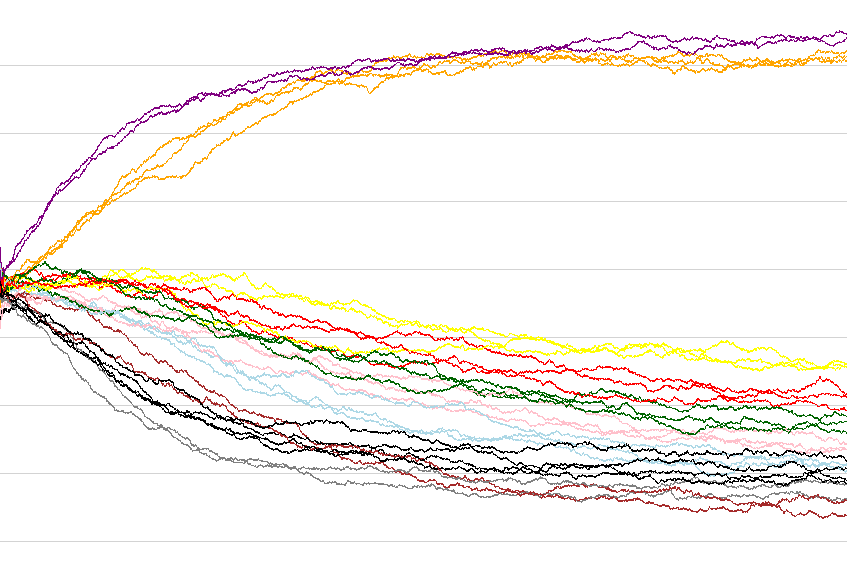
\includegraphics[width=\textwidth,height=4cm]{1.png}
\caption{The evolution of the genes controlling asset purchases over 600 generations and 400,000 games played.}
\label{fig:res1}
\end{figure*}


He we look at the average K-value of each gene across a population of \textbf{10,000} individuals. In this trial, we used a \textbf{random selection} crossover strategy, and ran the simulation for \textbf{400,000} games, resulting in a population with an average generation of 628. A chart of the values of K over the full simulation is given in Figure~\ref{fig:res1}, and the final K-values of the genes are listed in table~\ref{tab:res1}.

\begin{table}
\normalsize
\centering
\rowcolors{2}{gray!25}{white!50}
\begin{tabular}{*5l}    
\toprule
\textbf{Asset} & \textbf{K} \\ 
\midrule
Mayfair					 & 0.932 \\
Park Lane                & 0.929 \\
Vine Street              & 0.907 \\
Bow Street               & 0.898 \\
Marlborough Street       & 0.897 \\
Coventry Street          & 0.370 \\
Leicester Square         & 0.369 \\
Piccadilly               & 0.368 \\
The Strand               & 0.346 \\
Trafalgar Square         & 0.319 \\
Fleet Street             & 0.305 \\
Bond Street              & 0.281 \\
Oxford Street            & 0.271 \\
Regent Street            & 0.269 \\
Northumberland Avenue    & 0.250 \\
Pall Mall                & 0.227 \\
Whitehall                & 0.227 \\
Liverpool Street Station & 0.219 \\
Euston Road              & 0.211 \\
The Angel lslington      & 0.201 \\
Pentonville Road         & 0.200 \\
Fenchurch Street Station & 0.194 \\
Marylebone Station       & 0.190 \\
King's Cross Station     & 0.178 \\
Water Works              & 0.173 \\
Electric Company         & 0.148 \\
Old Kent Road            & 0.147 \\
Whitechapel              & 0.116 \\
\bottomrule
 \hline
\end{tabular}
\caption{The final K values of the asset-purchase genes after 600 generations and 400,000 games played.}
\label{tab:res1}
\end{table}

The most noticeable result is the the two purple assets (\textbf{Mayfair} and \textbf{Park Lane}) are the top two preferences; followed closely by the three orange assets (\textbf{Vine Street}, \textbf{Bow Street} and \textbf{Marlborough Street}). All the other assets are shunned in comparison, however there is some order among these. Thus, our population has evolved to significantly prefer the purple and orange assets. This is somewhat in line with our expectations, as it is easier to get a monopoly over the two purple properties and they earn high rent, while the orange properties are cheap but are more often landed on than any other colour.

%----------------------------------------------------------------------------------------------------
\section{Variation}
\label{sec:var}

Intro

\subsection{Population}

\subsection{Mutation Level}

\subsection{Granularity of Genes}



%----------------------------------------------------------------------------------------------------
\section{Conclusions} 
\label{sec:con}

Intro




\end{document}